\documentclass[11pt]{article}

\usepackage{epsfig}
\usepackage{amsfonts}
\usepackage{amssymb}
\usepackage{amstext}
\usepackage{amsmath}
\usepackage{xspace}
\usepackage{theorem}
\usepackage{hyperref}
\usepackage{fullpage}
\usepackage{enumitem}
\usepackage{graphicx}
\usepackage{indentfirst}

\usepackage{listings}

\usepackage{enumitem}                     


 \usepackage{titlesec}

\titleformat*{\section}{\bfseries}
\titleformat*{\subsection}{\bfseries}
\titleformat*{\subsubsection}{\bfseries}
\titleformat*{\paragraph}{\bfseries}
\titleformat*{\subparagraph}{\bfseries}


\newenvironment{proof}{{\bf Proof:  }}{\hfill\rule{2mm}{2mm}}
\newenvironment{proofof}[1]{{\bf Proof of #1:  }}{\hfill\rule{2mm}{2mm}}
\newenvironment{proofofnobox}[1]{{\bf#1:  }}{}
\newenvironment{example}{{\bf Example:  }}{\hfill\rule{2mm}{2mm}}


\newtheorem{fact}{Fact}[section]
\newtheorem{lemma}[fact]{Lemma}
\newtheorem{theorem}[fact]{Theorem}
\newtheorem{definition}[fact]{Definition}
\newtheorem{corollary}[fact]{Corollary}
\newtheorem{proposition}[fact]{Proposition}
\newtheorem{claim}[fact]{Claim}
\newtheorem{exercise}[fact]{Exercise}

% math notation
\newcommand{\R}{\ensuremath{\mathbb R}}
\newcommand{\Z}{\ensuremath{\mathbb Z}}
\newcommand{\N}{\ensuremath{\mathbb N}}
\newcommand{\F}{\ensuremath{\mathcal F}}
\newcommand{\SymGrp}{\ensuremath{\mathfrak S}}

\newcommand{\size}[1]{\ensuremath{\left|#1\right|}}
\newcommand{\ceil}[1]{\ensuremath{\left\lceil#1\right\rceil}}
\newcommand{\floor}[1]{\ensuremath{\left\lfloor#1\right\rfloor}}
\newcommand{\poly}{\operatorname{poly}}
\newcommand{\polylog}{\operatorname{polylog}}

% anupam's abbreviations
\newcommand{\e}{\epsilon}
\newcommand{\half}{\ensuremath{\frac{1}{2}}}
\newcommand{\junk}[1]{}
\newcommand{\sse}{\subseteq}
\newcommand{\union}{\cup}
\newcommand{\meet}{\wedge}

\newcommand{\prob}[1]{\ensuremath{\text{{\bf Pr}$\left[#1\right]$}}}
\newcommand{\expct}[1]{\ensuremath{\text{{\bf E}$\left[#1\right]$}}}
\newcommand{\Event}{{\mathcal E}}

\newcommand{\mnote}[1]{\normalmarginpar \marginpar{\tiny #1}}

\setenumerate[0]{label=(\alph*)}


%%%%%%%%%%%%%%%%%%%%%%%%%%%%%%%%%%%%%%%%%%%%%%%%%%%%%%%%%%%%%%%%%%%%%%%%%%%
% Document begins here %%%%%%%%%%%%%%%%%%%%%%%%%%%%%%%%%%%%%%%%%%%%%%%%%%%%
%%%%%%%%%%%%%%%%%%%%%%%%%%%%%%%%%%%%%%%%%%%%%%%%%%%%%%%%%%%%%%%%%%%%%%%%%%%



\begin{document}

\noindent {\large {\bf 601.465 / 601.665 Natural Language Processing} \hfill {{\bf Fall 2021}}}\\
{{\bf Homework \#1}} \hfill {Henry Li Xinyuan} \\

\section{Random Sentence Generator}

\subsection{Sample sentences}

\begin{enumerate}[label=(\arabic*)]
      \item every pickle in the president pickled the sandwich with the sandwich in every pickle under a president in a floor on every president !
      \item the sandwich kissed the delicious sandwich .
      \item every sandwich pickled the pickle !
      \item is it true that every sandwich under the president pickled a president ?
      \item is it true that a pickle wanted every sandwich in a chief of staff with a perplexed president under the chief of staff on the pickle under the chief of staff with every chief of staff on the sandwich in the pickle ?
      \item every delicious president pickled the president .
      \item is it true that a president in the delicious pickle on a chief of staff in every floor under a president with the president with the sandwich with a sandwich on a pickled sandwich on every pickled floor under every floor in every president in a chief of staff ate every sandwich ?
      \item a chief of staff kissed the floor .
\end{enumerate}

\subsection{Sample sentences with trees}
\subsubsection{}

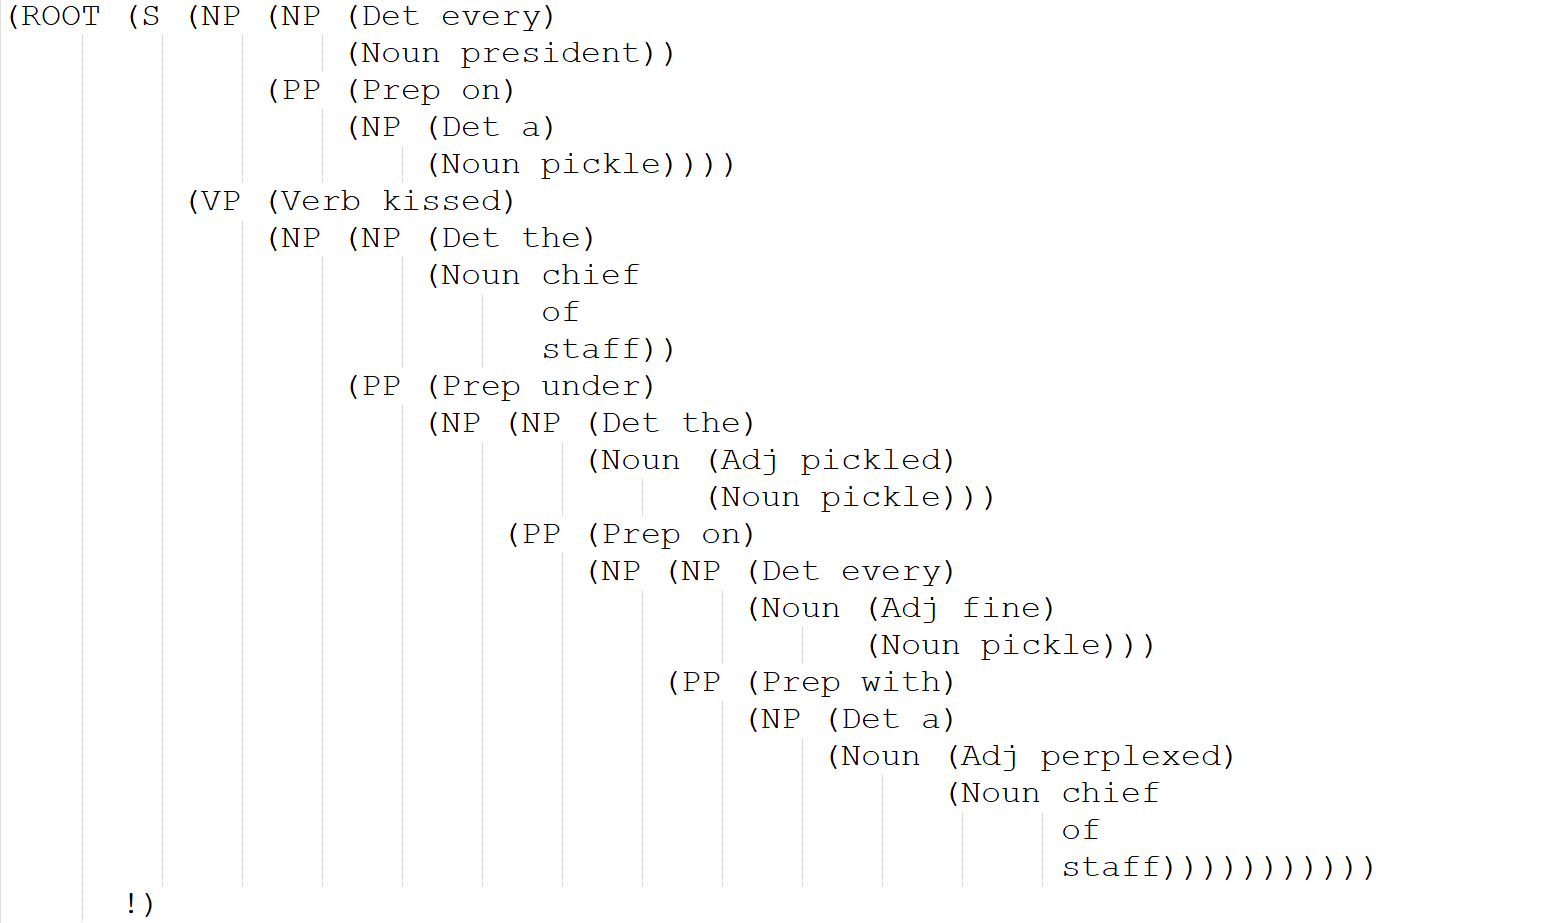
\includegraphics{tree1.png}

\noindent every president on a pickle kissed the chief of staff under the pickled pickle on every fine pickle with a perplexed chief of staff !

\subsubsection{}

\noindent a sandwich understood the pickle .
\medskip
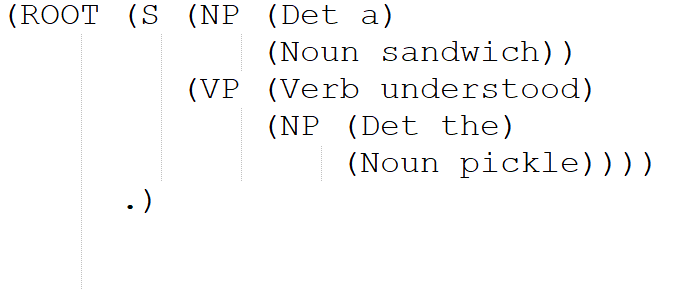
\includegraphics{tree2.png}

\subsection{Sample sentences with trees, with max 5 expansions}
\subsubsection{}

\noindent ... ... ... ... ... ... .
\medskip
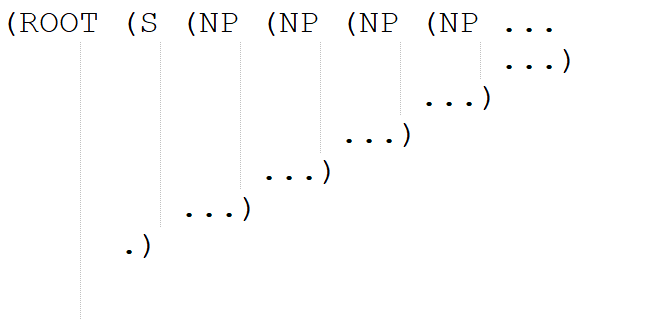
\includegraphics{tree3.png}

\subsubsection{}

\noindent the sandwich ... ... .
\medskip
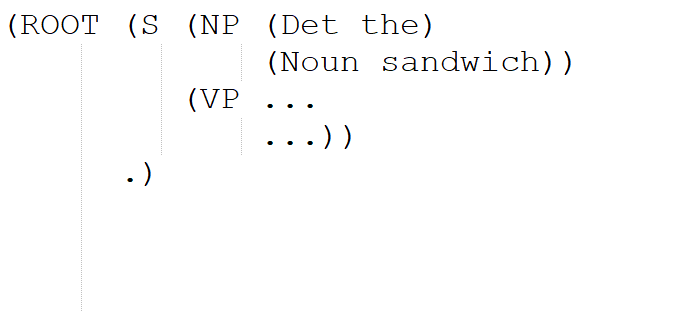
\includegraphics{tree4.png}

\section{Understanding Grammar Rules and Weights}

\subsection{Questions}

\subsubsection{}

\noindent Certain rules allow for large recursive structures to be generated. Some of the rules in question include:

\begin{enumerate}[label=(\arabic*)]
      \item Noun -> Adj Noun

            ... delicious delicious president ...
      \item NP -> NP PP and PP -> Prep NP

            ... delicious president in delicious president in delicious president ...

            \noindent In actual speech, we don't tend to modify our nouns with more adjectives than necessary, for doing so may compromise clarity. While it might be tempting to do so in writing as a means of avoiding long expositions, We can think of very few examples of writers employing such a technique. Likewise, while long chains of preposition structures are allowed grammatically and can exist conceptually, it is far more common for each link in the chain to be introduced separately, only for their relationship to be unveiled later.
\end{enumerate}

\subsubsection{}

\noindent The rule which allow for multiple modifying adjectives (Noun -> Adj Noun) has a probability of $1/6$ to be used as the substitution rule for a Noun symbol. The probability of having more than $3$ adjectives modifying a single noun is therefore only $1/216$ or less than $0.5\%$. By contrast, the rule which results in long preposition chains has a $50\%$ chance of being employed whenever an NP symbol appears.

\subsubsection{}

\noindent We need to modify the weights of the two rules mentioned in part $2.1.1$, decreasing the weight of "NP -> NP PP" while increasing the weight of "Noun -> Adj Noun". While the latter situation may appear at an acceptable frequency by our standard, subsequent increases in the size of the Noun vocabulary would tip that balance towards fewer adjectives. For the purpose of this exercise, We changed the weight of "NP -> NP PP" to $0.1$ while increasing the weight of "Noun -> Adj Noun" to $2$. Below are some of the sentences generated with the new grammar:

\begin{enumerate}[label=(\arabic*)]
      \item is it true that the fine sandwich pickled every pickled president ?
      \item every floor pickled every pickle !
      \item is it true that the pickled fine sandwich understood the sandwich ?
      \item a floor pickled the floor !
      \item a perplexed president kissed every president !
\end{enumerate}

\subsubsection{}

\noindent Below are some of the changes We made to grammr2, as well as our reasoning for each.

\begin{enumerate}[label=(\arabic*)]
      \item Change the weight of "Det -> every" from $1$ to $0.2$

            We don't tend to make general statements nearly as often as we do statement about individual people/ojbects.

      \item Reduce the weight of "ROOT -> is it true that S ?" from $1$ to $0.1$; reduce the weight of "ROOT -> S !" from $1$ to $0.2$.

            We are far more likely to make assertions than to ask about their veracity. We also don't exclaim nearly as often as we speak in a neutral tone.

      \item Make the following changes to the weight of verb terminals: "Verb -> wanted" from $1$ to $2$, "Verb -> kissed" from $1$ to $0.2$, "Verb -> understood" from $1$ to $2$, "Verb -> pickled" from $1$ to $0.1$

            These are hopefully better reflections of the relative frequency of these verbs.
\end{enumerate}

\noindent We found no issues with the relative weights of other substitutions (Adj, Prep, Noun, "a" vs. "the").

\subsubsection{}

\noindent Some examples of sentences generated under the revised grammar:

\begin{enumerate}[label=(\arabic*)]
      \item a pickle wanted the sandwich under a perplexed perplexed pickle .
      \item a floor understood the sandwich .
      \item the president understood the perplexed floor !
      \item a sandwich ate the pickle .
      \item a sandwich understood the fine sandwich !
      \item a perplexed fine perplexed president in the chief of staff kissed the pickle .
      \item is it true that the delicious floor ate a president ?
      \item every delicious sandwich in a pickle understood a president !
      \item a pickle ate a floor .
      \item a pickle on the president wanted the perplexed floor .
\end{enumerate}

\subsection{Grammar Modification}

\noindent Please refer to grammar3.gr for a full list of revised substitution rules. In order to stay consistent with the capitalised - non-terminal, uncapitalised - terminal rule set out earlier on in the handout, names do not have their first letter capitalised. The sample sentences can be generated in the revised grammar with the following expansion trees:

\begin{enumerate}[label=(\arabic*)]
      \item "Sally ate a sandwich ."

            \begin{verbatim}
(ROOT (S (NP (Name Sally))
         (VP (Verb_Transivite ate)
             (NP (Det the)
                 (Noun sandwich))))
      .)
      \end{verbatim}

      \item "Sally and the president wanted and ate a sandwich ."

            \begin{verbatim}
(ROOT (S (NP (NP (Name Sally))
             and
             (NP (Det the)
                 (Noun president)))
         (VP (Verb_Transivite (Verb_Transivite wanted)
                               and
                               (Verb_Transivite ate))
             (NP (Det a)
                 (Noun sandwich))))
      .)
\end{verbatim}

      \item "the president sighed ."

            \begin{verbatim}
(ROOT (S (NP (Det the)
             (Noun president))
         (VP (Verb_Intransitive sighed)))
      .)
\end{verbatim}

      \item "the president thought that a sandwich sighed ."

            \begin{verbatim}
(ROOT (NP (Det the)
          (Noun president))
      (V_C (Verb_Conjunctive thought)
           that)
      (S (NP (Det a)
             (Noun sandwich))
         (VP (Verb_Intransitive sighed)))
      .)
\end{verbatim}

      \item "it perplexed the president that a sandwich ate Sally ."

            \begin{verbatim}
(ROOT it
      (Verb_Transitive_Emotive perplexed)
      (NP (Det the)
          (Noun president))
      that
      (S (NP (Det a)
             (Noun sandwich))
         (VP (Verb_Transitive ate)
             (NP (Name sally))))
      .)
\end{verbatim}

      \item "that a sandwich ate Sally perplexed the president ."

            \begin{verbatim}
(ROOT that
      (S (NP (Det a)
             (Noun sandwich))
         (VP (Verb_Transitive ate)
             (NP (Name sally))))
      (Verb_Transitive_Emotive perplexed)
      (NP (Det the)
          (Noun president))
      .)
\end{verbatim}

      \item "the very very very perplexed president ate a sandwich ."

            \begin{verbatim}
(ROOT (S (NP (Det the)
      (Noun (Adj (Adv very)
                 (Adj (Adv very)
                      (Adj (Adv very)
                           (Adj perplexed))))
            (Noun president)))
      (VP (Verb_Transitive ate)
          (NP (Det a)
              (Noun sandwich))))
      .)
\end{verbatim}

      \item "the president worked on every proposal on the desk ."

            \begin{verbatim}
(ROOT (S (NP (Det the)
             (Noun president))
         (VP (Verb_Transitive worked
                              on)
             (NP (NP (Det every)
                     (Noun proposal))
                 (PP (Prep on)
                     (NP (Det the)
                         (Noun desk))))))
      .)
            \end{verbatim}
\end{enumerate}

\noindent We prefer doing a bit more legwork and making our code more readable at surface-level, thus sub-categories will not be abbreviated and will follow the main categories, separated by an underscore.

\subsection{Questions continued}

\subsubsection{}

Some of the significant changes in grammar3 are listed here:

\begin{enumerate}[label=(\arabic*)]
      \item Added new sentence structures which don't follow the s -> NP VP pattern. 
      
\begin{verbatim}
0.2 ROOT    NP V_C S .
0.2 ROOT    it Verb_Transitive_Emotive NP that S .
0.2 ROOT    that S Verb_Transitive_Emotive NP .
\end{verbatim}
      The first of these rules handles sentences joined together by conjunctive verbs; The second and the third handle the instances where an sentence acts as the subject acting on the object with an emotive transitive verb.
      \item Added a new class of words - adverbs, which can be used to modify adjectives.
      \item Subdivided verbs into Verb\_Transitive, Verb\_Intransitive, and Verb\_Conjunctive.
      \item Added a sub-category of Verb\_Transivite: Verb\_Transitive\_Emotive, which are verbs which can describe the emotive effect on the object.
      \item Added a new pre-terminal tag "Name", which are nouns that have no article attached to them. Added a rule where "NP" can be replaced by "Name".
\end{enumerate}

\subsubsection{}

Below are some of the example sentences generated with grammar3:

\begin{enumerate}[label=(\arabic*)]
      \item a spectre and the perplexed desk and a fine pickled desk and the delicious delicious delicious spectre and a delicious floor under a desk and a desk in a president thought that a chief of staff understood .
      \item a sandwich believed that a dauntingly pickled perplexed floor wanted the sandwich .
      \item the pickle shouted .
      \item the fine chief of staff wanted every president .
      \item that the sandwich understood a pickle worried marx .
      \item that a president wanted the delicious president worried the pickle .
      \item the desk ate and understood the desk .
      \item a desk understood that the pickle understood the spectre .
      \item that the fine chief of staff pickled the pickle worried europe .
      \item it worried the chief of staff that the chief of staff and a chief of staff and sally understood sally .
\end{enumerate}

\section{Sentence Ambiguity and Parsing}

\subsection{Questions}

\subsubsection{}

\noindent The other possible derivation is as follows:

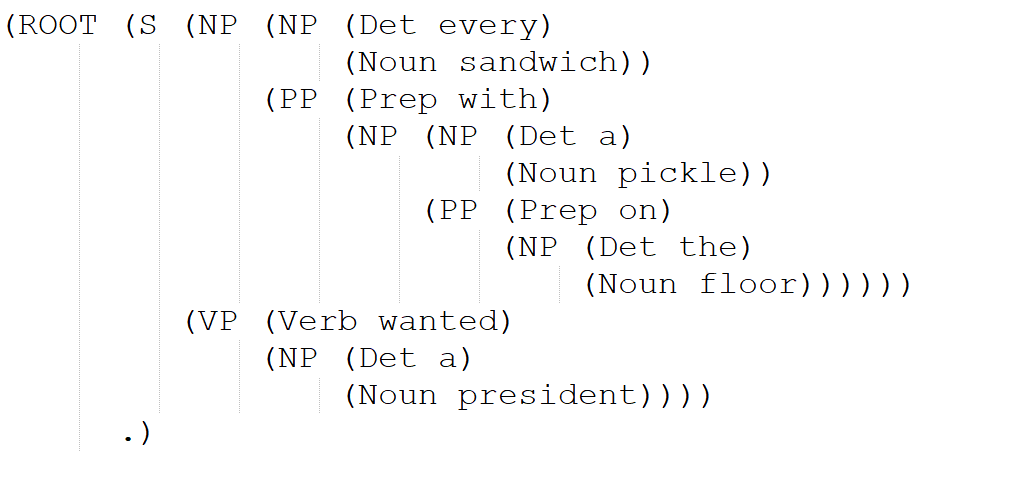
\includegraphics{tree5.png}

This derivation results in a different interpretation of the same sentence. In the original, the subject is every sandwich with a pickle, which are on the floor. In the new interpretation, the subject is every sandwich which have a pickle on the floor.

\subsection{Parsers}

The example sentences from part $2.2$ were tested through the parser, with the correct ones being approved or rejected.

\subsection{Questions continued}

\subsubsection{}

Below are some sentences generated through grammar3, their original derivation tree, and the derivation tree recovered by the parser.

\begin{enumerate}[label=(\arabic*)]
      \item a spectre shouted !

            Original derivation:
            \begin{verbatim}
(ROOT (S (NP (Det a)
             (Noun spectre))
         (VP (Verb_Intransitive shouted)))
      !)
      \end{verbatim}

            Parsed derivation:
            \begin{verbatim}
(ROOT (S (NP (Det a)
             (Noun spectre))
         (VP (Verb_Intransitive shouted)))
      !)
      \end{verbatim}
      \item the president wanted henry .

            \begin{verbatim}
(ROOT (S (NP (Det the)
             (Noun president))
         (VP (Verb_Transitive wanted)
             (NP (Name henry))))
      .)
      \end{verbatim}

            Parsed derivation:
            \begin{verbatim}
(ROOT (S (NP (Det the)
             (Noun president))
         (VP (Verb_Transitive wanted)
             (NP (Name henry))))
      .)
      \end{verbatim}
      \item henry understood a spectre .

            \begin{verbatim}
(ROOT (S (NP (Name henry))
             (VP (Verb_Transitive understood)
             (NP (Det a)
                 (Noun spectre))))
      .)
      \end{verbatim}

            Parsed derivation:
            \begin{verbatim}
(ROOT (S (NP (Name henry))
         (VP (Verb_Transitive understood)
             (NP (Det a)
                 (Noun spectre))))
      .)
      \end{verbatim}
      \item is it true that a chief of staff wanted a proposal ?

            \begin{verbatim}
(ROOT is
      it
      true
      that
      (S (NP (Det a)
             (Noun chief
                   of
                   staff))
         (VP (Verb_Transitive wanted)
             (NP (Det a)
                 (Noun proposal))))
      ?)
      \end{verbatim}

            Parsed derivation:
            \begin{verbatim}
(ROOT is
      it
      true
      that
      (S (NP (Det a)
             (Noun chief
                   of
                   staff))
         (VP (Verb_Transitive wanted)
             (NP (Det a)
                 (Noun proposal))))
      ?)
      \end{verbatim}
      \item the pickle in a president in a fine pickle in sally heard and understood that a pickle shouted .

            \begin{verbatim}
(ROOT (NP (NP (NP (Det the)
                  (Noun pickle))
              (PP (Prep in)
                  (NP (Det a)
                      (Noun president))))
              (PP (Prep in)
                  (NP (NP (Det a)
                          (Noun (Adj fine)
                                (Noun pickle)))
                      (PP (Prep in)
                          (NP (Name sally))))))
      (V_C (Verb_Conjunctive (Verb_Conjunctive heard)
                             and
                            (Verb_Conjunctive understood))
           that)
      (S (NP (Det a)
             (Noun pickle))
         (VP (Verb_Intransitive shouted)))
      .)
      \end{verbatim}

            Parsed derivation:
            \begin{verbatim}
(ROOT (NP (NP (Det the)
              (Noun pickle))
          (PP (Prep in)
              (NP (NP (NP (Det a)
                          (Noun president))
                      (PP (Prep in)
                          (NP (Det a)
                              (Noun (Adj fine)
                                    (Noun pickle)))))
              (PP (Prep in)
                  (NP (Name sally))))))
      (V_C (Verb_Conjunctive (Verb_Conjunctive heard)
                             and
                             (Verb_Conjunctive understood))
           that)
      (S (NP (Det a)
             (Noun pickle))
         (VP (Verb_Intransitive shouted)))
      .)
      \end{verbatim}
\end{enumerate}

Of the five sentences listed above, only one has any potential to cause any confusion (number $5$), and sure enough it does. The reason for this confusion is the same as for the example given in part $3.1$. The same principle can be extended to all sentences that contain any kind of recursive structures which can contain multiple copies of itself (ie., an NP can be expanded into two parts, each containing an NP).

\subsubsection{}

In total there are $5$ different ways to interpret the given phrase:

\begin{enumerate}[label=\arabic*]
      \item (((every sandwich with a pickle) on the floor) under the chief of staff)
      \item ((every sandwich with a pickle) on (the floor under the chief of staff))
      \item ((every sandwich with (a pickle on the floor)) under the chief of staff)
      \item (every sandwich with ((a pickle on the floor) under the chief of staff))
      \item (every sandwich with (a pickle on (the floor under the chief of staff)))
\end{enumerate}

At each iteration, some pair adjacent noun phrases need to be chosen to be the next ones that would be combined into a NP PP structure. At the first iteration there are $4$ NPs and therefore $3$ different possible combinations. Finally, one of the $3 \times 2 = 6$ combinations is a duplicate.

The following command confirms that there are exactly $5$ parses for the above phrase:

\begin{verbatim}
perl HW1/parse -g HW1/grammar.gr -c -s NP

# number of parses = 5
\end{verbatim}

\subsubsection{}

We look at a few sentences that were generated with the original grammar:

\begin{enumerate}[label=(\arabic*)]
      \item every floor with every floor pickled the floor .

            Number of parses $= 1$.
      \item every floor with every floor with every floor pickled the floor .

            Number of parses $= 2$.
      \item every floor with every floor with every floor with every floor pickled the floor .

            Number of parses $= 5$.
      \item every floor with every floor with every floor with every floor with every floor pickled the floor .

            Number of parses $= 14$.

      \item every floor with every floor with every floor with every floor with every floor with every floor pickled the floor .

            Number of parses $= 42$.
\end{enumerate}

As mentioned in part $3.3.1$, ambiguity arises in sentences generated from grammar.gr when long strings of consecutive PPs occur. Assuming that only one such string appears in a sentence, the number of different parses is decided by the length of the string: specifically, the number of parses is equal to the value of the Catalan number sequence on the index given by the length of the string of PPs. In the case where multiple disjoint strings of PPs exist, we can observe the following pattern:

\begin{enumerate}[label=(\arabic*)]
      \item every floor with every floor with every floor with every floor pickled the floor with the floor .

            Number of parses $= 5 = 5 \times 1$.

      \item every floor with every floor with every floor with every floor pickled the floor with the floor with the floor .

            Number of parses $= 10 = 5 \times 2$.

      \item every floor with every floor with every floor with every floor pickled the floor with the floor with the floor with the floor .

            Number of parses $= 25 = 5 \times 5$.
\end{enumerate}

We can observe (and easily see why) the number of parses is equal to the product of the number of parses of each PP sequence, which in turn is derived from the Catalan number sequence and the length of each PP sequence. Now because grammar.gr would not generate sentences with more than $2$ PP sequences, the number of parses for a sentence generated from grammar.gr is at most the product of two numbers. On first look it seems that this would not be the case for the revised grammar3 though, which allows for NPs to be concatenated alongside each other, each of which can then be collapsed into a long, ambiguous PP sequence. However this would turn out not to be the case, as we can see with the following sentence:

\begin{verbatim}
every floor with every floor with every floor with every floor and henry 
pickled the floor with the floor .
\end{verbatim}

The number of parses for this sentence is $14$ and not $5$, because the phrase "and henry" could be bundled with any NP preceding it just like a PP could, thus acting just like a PP in a PP sequence. Similarly, the sentence 

\begin{verbatim}
every floor with every floor with every floor with every floor and henry 
in henry in henry in henry pickled the floor with the floor with the floor with the floor .
\end{verbatim}

has $2145 = 429 \times 5$ parses, with $429$ being the $8$th instance of the Catalan numbers and the length of the first NP-PP sequence in the sentence..

Note that in grammar3, verbs can be concatenated with each other too. They can't be bundled together with NPs, but the way the concatenation rules are written now (V and V), they can be joined in pairs similar to NPs can. An example would be the sentence 

\begin{verbatim}
henry ate and ate and ate and ate .
\end{verbatim}

which has $5$ parses.

\subsubsection{}

\begin{enumerate}
      \item The probability denoted by $p(best\_parse)$ is the product of all the normalised (with respect to all possible expansions of a symbol) probability of each expansion step from ROOT to the expanded sentence. While the weight assigned to each expansion can be quite large (at least $1$ in the case of grammar.gr), after normalisation their values fall substantially. 
      
      The reason $p(sentence) = p(best\_parse)$ is because there is only one possible parse for the sentence in question.

      The third number $1$ is just as it is labeled: $p(best\_parse | sentence)$, or $p(best\_parse \cap sentence) / p(sentence)$, or the probability of parsing this sentence in the most probable way given the sentence.

      \item The third number $.5$ tells us that it is equally probable for the sentence to be parsed in the most probable way, or for it to be parsed in some other way(s). As we've discussed earlier, the ambiguity in this sentence arises from whether we read "every sandwich with a pickle" first or "a pickle on the floor" first. To understand why its value is exactly $.5$, we can either expand both expansions out completely and see that their probability are the product of the same normalised probabilities, just with the expansions coming in a different order. We can also use the intuition that at the crucial intersection which would bring ambituity (do we expand the NP in "every sandwich with NP" into an NP PP pattern or not) has exactly $.5$ probability.
      
      \item A cross-entropy measures how "surprised" the parser would be at the corpus, given the grammar. In order to normalise the result, the total cross-entropy of the input is divided by the number of words in the input. The value $-43.833$ is given by summing the product of the probability of each possible parse of each sentence given the sentence, multiplied with the corresponding probability of each parse (in general). In other words, $\log(5.144e-005) + .5 \times \log(1.240e-009) + 0.5 \times \log(1.240e-009)$.
      
      \item The perplexity can be calculated by $2^{cross-entropy} = 2^{2.435} = 5.408$.
      
      \item It is impossible to generate "the president ate ." under grammar.gr. As such, both $p(best\_parse)$ ($0/0$) and $p(best\_parse \cap sentence) / p(sentence)$ are undefined. In some systems, undefined values could be treated as $0$, resulting in a $log(0)$ term which converges to $-inf$ (although in the parse script, this is done explicitly). Thus the cross-entropy of the sentence, and therefore the corpus, is infinite.
\end{enumerate}

\subsubsection{}

\begin{enumerate}
      \item The pipe we used to calculate the average cross-entropy of grammar2 is as follows:
      
      \begin{verbatim}
py randsent.py -g grammar2.gr -n 100000 | perl parse -g grammar2.gr -P -c
      \end{verbatim}

      The per-word cross-entropy of the $100000$ sentences turned out to be $1.930$ bits. We repeated this a few times with varying sample sizes and generally achieved similar results.

      A small concern was the possibility that one of these $100000$ sentences could have gone above the expansion limit and caused the cross-entropy to be infinite. Fortunately it didn't happen in this case.

      \item Our hypothesis is that grammar3 would have a much larger per-word cross-entropy, due to its much larger vocabulary and more varied sentence structure. As such, we ran the following command: 
      
      \begin{verbatim}
py randsent.py -g grammar3.gr -n 100000 | perl parse -g grammar3.gr -P -c
      \end{verbatim}

      The parse script reported a per-word cross-entropy of $2.563$ bits, which is indeed much higher than the value reported for grammar2

      \item The issue that had been forseen in part (a) occurs to us, with some sentences going above the expansion limit and the cross entropy reported as infinite.

\end{enumerate}

\subsubsection{}

We will use the following commands to evaluate the ability of the three grammars to predict a corpus generated from grammar2, and then we will compare the results:

\begin{verbatim}
py randsent.py -g grammar2.gr -n 100000 | perl parse -g grammar1.gr -P -c
py randsent.py -g grammar2.gr -n 100000 | perl parse -g grammar3.gr -P -c
\end{verbatim}

grammar.gr had a cross-entropy of $2.290$ bits per word when trying to predict grammar2, while grammar3 had a cross-entropy per word of $2.366$ bits. These results support the above hypothesis.

We also observe a lower cross-entropy when grammar3 predicts a corpus generated from grammr2 than when grammar3 predicts a corpus generated from itself. This is to be expected as grammar2 is a strict subset of grammar3.

\section{Extending the Grammar}

\begin{enumerate}
      \item Recall that the grammars that we're dealing with are "context-free", meaning the way each symbol gets expanded is completely independent from any other symbol. As such, we would need to decide whether the first syllable following the determiner has no leading consonant prior to breaking down the NP into Det Noun. That information would then need to be retained throughout the pipe as the noun phrase gets broken down.
      
      What we did to achieve this are the following: we re-label each Noun, Adj and Adv into either Noun\_C, Adj\_C, Adv\_C or Noun\_V, Adj\_V, Adv\_V:
      
\begin{verbatim}
1   Noun_C	president
1   Noun_C	sandwich
1   Noun_V  orange
\end{verbatim}
      
      We add rules which convert a Noun into either a Noun\_C or a Noun\_V (much higher weight for Noun\_C), likewise for Adj and Adv:

\begin{verbatim}
1   Noun    Noun_C
0.1 Noun    Noun_V
\end{verbatim}
      
      We also split determiners into D\_C and D\_V following the same procedure. Finally, we now add a class MN (modified nouns), which are nouns that may be modified by adjectives (which in turn may be modified by adverbs) without articles. Natually MN comes in two different flavours, MN\_C and MN\_V, depending on its starting syllable. We now expand each NP into D\_C MN\_C or D\_V MN\_V. MN\_C can then be expanded by MN\_C -> Adj\_C MN or MN\_C -> Noun\_C:

\begin{verbatim}
1   NP      D_C MN_C
2   MN_C    Adj_C MN
0.5 Adj_C   Adv_C Adj
1   MN_C    Noun_C
\end{verbatim}

      For the purpose of future scalability, we also subdivided determiners by whether they are definite or indefinite articles.

      The above mentioned changes has allowed us to generate the following sentence:

\begin{verbatim}
an incredibly fine floor and a pickled magnificently pickled pickled chief of staff 
understood !

(ROOT (S (NP (NP (D_I_V an)
                 (MN_V (Adj_V (Adv_V incredibly)
                              (Adj (Adj_C fine)))
                       (MN (Noun (Noun_C floor)))))
             and
             (NP (D_I_C a)
                 (MN_C (Adj_C pickled)
                       (MN (MN_C (Adj_C (Adv_C magnificently)
                                        (Adj (Adj_C pickled)))
                                 (MN (MN_C (Adj_C pickled)
                                           (MN (Noun (Noun_C chief
                                                             of
                                                             staff))))))))))
         (VP (Verb_Intransitive understood)))
      !)
\end{verbatim}

      Note that this expansion is generated from grammar3.5, since the expansion from grammar4 would be too wide to include in this document.

      \item The simplest yes or no question is one which has the same sentence structure as a statement, but spoken with a rising tone:
      
\begin{verbatim}
a spectre haunted Europe ?
\end{verbatim}

      One may argue that such a sentence is grammatically incorrect, but it gets spoken often enough that we believe it deserves a place in the dictionary.

\begin{verbatim}
0.05    ROOT    S ?
\end{verbatim}

      In order to construct grammatically correct questions, we must start paying attention to verb tense. We will tag each verb category with one of five tenses (Present, Past, PresentParticiple, PastParticiple). We also want a new category of verbs: Verb\_Auxiliary, which consists of the words that one would lead a sentence with when constructing a yes or no question (do, does, will, is, etc.).

      We observe that the auxiliary verbs have a dependency on the subject, depending on whether the subject is third-person singular(does he vs. do they), or whether the subject is first or second-person (am I vs. are you vs. is he). As such, it becomes necessary to keep track of these properties in our noun phrases.

      We also observe that in the partial sentence following the auxiliary verb, the verb would need to be conjugated to different forms tenses depending on the subject and the auxiliary verb. As such, we have to propogate whether a verb has a third-person singular subject, as well as the tense of the verb. By the time that a satisfactory system has been built for this purpose, we find ourselves equipped with the infrastructure to implement general verb tenses.

      Some of the rules that were introduced in this process are listed as follows:

\begin{verbatim}
0.2     ROOT    Q_YesOrNo ?

1   Q_YesOrNo   Verb_Auxiliary_Present_NoneThirdSingular NP_NoneThirdSingular 
VP_Present_NoneThirdSingular
1   Q_YesOrNo   Verb_Auxiliary_Present NP VP_Present_NoneThirdSingular
1   Q_YesOrNo   Verb_Auxiliary_Present_ThirdSingular NP_ThirdSingular 
VP_Present_NoneThirdSingular
\end{verbatim}

      For the sake of brevity, we will not include rules which propagate Verb, NP and VP properties. These additional rules have allowed us to generate sentences such as the following:

\begin{verbatim}
does the pickle want Henry ?
do Europe and the delicious angry orange and the president and the perplexed sandwich 
and a perplexed fine orange sleep ?
will Henry and Henry and the floor and the sandwich enrage Henry ?
am I asking for Henry ?
\end{verbatim}

      For reference, we attach the expansion tree of our last example:

\begin{verbatim}
(ROOT (Q_YesOrNo (Verb_Auxiliary_PresentParticiple_FirstPerson am)
                 I
                 (VP_PresentParticiple (Verb_Transitive_PresentParticiple asking
                                                                          for)
                                       (NP_Object (Name Henry))))
      ?)
\end{verbatim}

      \item Not implemented.
      \item Not implemented.
      \item While it could be said that this part is similar to part (a), it must be pointed out that part (b) forces the implementation of most of what is required for this part. English also fortunately has few morphology rules between nouns and other parts of a sentence: whether the subject is third-person singular forces a verb conjugation, whereas the singularity of objects does not interact with the rest of the sentence at all.

      Some of the key rules in implementing this part are shown here:

\begin{verbatim}
1   NP  NP_ThirdSingular

1   NP_ThirdSingular      D_Definite MN
1   NP_ThirdSingular      D_Indefinite_Consonant MN_Consonant
0.1 NP_ThirdSingular      D_Indefinite_Vowel MN_Vowel

1   NP_Subject_ThirdSingular    D_Definite MN
1   NP_Subject_ThirdSingular    D_Indefinite_Consonant MN_Consonant
0.1 NP_ThirdSingular            D_Indefinite_Vowel MN_Vowel

1   NP                              NP_NoneThirdSingular
1   NP_NoneThirdSingular            NP_ThirdSingular and NP_ThirdSingular
1   NP_NoneThirdSingular            NP_NoneThirdSingular and NP_ThirdSingular
1   NP_NoneThirdSingular            NP_ThirdSingular and NP_NoneThirdSingular
1   NP_NoneThirdSingular            NP_NoneThirdSingular and NP_NoneThirdSingular
1   NP_Subject_NoneThirdSingular    NP_Subject_ThirdSingular and NP_Subject_ThirdSingular
\end{verbatim}

      This is just a small peek of some of the new rules leading to the singular/plural split. Unfortunately the data structure of our grammar files are not very well-suited for writing expansion rules succintly: a tree structure, or a system which stores each trait as a label and allows each class to have multiple labels, would be much better for the current purpose.

      Some sentences which demonstrate grammar4's ability to maintain singular-plural consistency:

\begin{verbatim}
the spectre understands that a pickled orange understands Europe .
the pickled orange and a proposal understand Marx !
\end{verbatim}

      Of course we don't just want concatenated plural noun phrases, but also multiple copies of the same noun:

\begin{verbatim}
the pickles eat !
(ROOT (S (NP_Subject_Plural (D_Definite_Plural the)
                            (MN_Plural (Noun_Plural pickles)))
         (VP_Present_NoneThirdSingular (Verb_Intransitive_Present_NoneThirdSingular eat)))
      !)
\end{verbatim}

      Finally, we also added a new class of vocabulary: numbers. They can act as determiners for plural nouns. An example involving a number:

\begin{verbatim}
two sandwiches shout !
(ROOT (S (NP_Subject_Plural (D_Indefinite_Plural (Number_Plural two))
                            (MN_Plural (Noun_Plural sandwiches)))
         (VP_Present_NoneThirdSingular (Verb_Intransitive_Present_NoneThirdSingular shout)))
      !)
\end{verbatim}

      \item As we mentioned in part (b), a lot of the infrastructure for this part has been laid down. Some of the example sentences in previous parts already give a sneak peak of the grammar's ability to handle different tenses.
      
      Unfortunately this part is not fully implemented. The reason for this is that each additional verb form requires the entire verb vocabulary to be copied and revised. The size of the vocabulary we're using comes back to bite us here.

      Of the tenses that were listed on the handout, no perfect tenses where implemented; no future tenses were implemented except for the simple future tense.

      Two example sentences, along with their expansion trees, are listed as follows:

\begin{verbatim}
Sally had been haunting Henry .
(ROOT (S_PresentParticiple (NP_Subject (Name Sally))
                           had
                           been
                           (VP_PresentParticiple (Verb_Transitive_PresentParticiple haunting)
                                                 (NP_Object (Name Henry))))
      .)
a spectre is haunting Europe !
(ROOT (S_PresentParticiple (NP_Subject_ThirdSingular (D_Indefinite_Consonant a)
                                                     (MN_Consonant (Noun_Consonant spectre)))
                           is
                           (VP_PresentParticiple (Verb_Transitive_PresentParticiple haunting)
                                                 (NP_Object (Name Europe))))
      !)
\end{verbatim}

      \item Not implemented.

\end{enumerate}

\section{Extra Credit: Extending Further!}

Please refer to grammar4. It is a common fallacy for a builder, when putting down the simplest of blocks, to dream of something greater and grander, to leave the door open for the hut to grow into an edifice, only to step away onto greener pastures and never return to finish what had been started. In the construction of grammar4, elegance was sacrificed to allow for the grammar to not only be immediately human-readable, but also to ensure that the grammar would be highly robust and sensitive to grammatical, or even semantic, nuances. It therefore pains us greatly that the time we were alloted was insufficient for us to fulfill this grammar's potential. In addition, as we pointed out earlier, context-free grammars ultimately proved unsuitable for capturing the sentence-level morphology of the English language, the latter necessitating the introduction of unwieldly complexities in our otherwise pristinely structured grammar.

\end{document}